% This is "sig-alternate.tex" V2.0 May 2012
% This file should be compiled with V2.5 of "sig-alternate.cls" May 2012
%
% This example file demonstrates the use of the 'sig-alternate.cls'
% V2.5 LaTeX2e document class file. It is for those submitting
% articles to ACM Conference Proceedings WHO DO NOT WISH TO
% STRICTLY ADHERE TO THE SIGS (PUBS-BOARD-ENDORSED) STYLE.
% The 'sig-alternate.cls' file will produce a similar-looking,
% albeit, 'tighter' paper resulting in, invariably, fewer pages.
%
% ----------------------------------------------------------------------------------------------------------------
% This .tex file (and associated .cls V2.5) produces:
%       1) The Permission Statement
%       2) The Conference (location) Info information
%       3) The Copyright Line with ACM data
%       4) NO page numbers
%
% as against the acm_proc_article-sp.cls file which
% DOES NOT produce 1) thru' 3) above.
%
% Using 'sig-alternate.cls' you have control, however, from within
% the source .tex file, over both the CopyrightYear
% (defaulted to 200X) and the ACM Copyright Data
% (defaulted to X-XXXXX-XX-X/XX/XX).
% e.g.
% \CopyrightYear{2007} will cause 2007 to appear in the copyright line.
% \crdata{0-12345-67-8/90/12} will cause 0-12345-67-8/90/12 to appear in the copyright line.
%
% ---------------------------------------------------------------------------------------------------------------
% This .tex source is an example which *does* use
% the .bib file (from which the .bbl file % is produced).
% REMEMBER HOWEVER: After having produced the .bbl file,
% and prior to final submission, you *NEED* to 'insert'
% your .bbl file into your source .tex file so as to provide
% ONE 'self-contained' source file.
%
% ================= IF YOU HAVE QUESTIONS =======================
% Questions regarding the SIGS styles, SIGS policies and
% procedures, Conferences etc. should be sent to
% Adrienne Griscti (griscti@acm.org)
%
% Technical questions _only_ to
% Gerald Murray (murray@hq.acm.org)
% ===============================================================
%
% For tracking purposes - this is V2.0 - May 2012

%\documentclass{acm_proc_article-sp}
\documentclass{sig-alternate}
\usepackage{color}
\usepackage{multirow}
\usepackage{listings}
\usepackage{url}

\lstset{language=java, numbers=left, numberstyle=\tiny\color{black}, numbersep=3pt, escapeinside={\$}, basicstyle=\footnotesize\ttfamily, escapeinside={\%*}{*)}}

\newif\ifdraft
\drafttrue
%\draftfalse                                                                              
\ifdraft
\newcommand{\zhaonote}[1]{{\textcolor{cyan}    { ***Zhao:      #1 }}}
\newcommand{\note}[1]{ {\textcolor{red}    {\bf #1 }}}
\else
\newcommand{\zhaonote}[1]{}
\newcommand{\note}[1]{}
\fi


\begin{document}

\title{Gineala: Diagnosing Data with Machine Learning Pipeline Lineage}

\numberofauthors{3} 
\author{
% 1st. author
\alignauthor Zhao~Zhang\\\
       \affaddr{AMPLab}\\
       \affaddr{University of California, Berkeley} \\
       \email{zhangzhao@berkeley.edu}    
% 4th. author       
\alignauthor Evan~Sparks\\\
       \affaddr{AMPLab}\\
       \affaddr{University of California, Berkeley}\\
       \email{sparks@berkeley.edu}       
% 6th. author
\alignauthor Michael~J.~Franklin\\
       \affaddr{AMPLab}\\
       \affaddr{University of California, Berkeley}\\
       \email{franklin@berkeley.edu}   
}

\maketitle

\begin{abstract}
We present the Gineala lineage system as part of the KeystoneML machine learning pipeline to provide
users the capability of end-to-end data investigation. 
Practically, users can better understand the machine learning process and results with such analysis.
They can also possibly identify and remove data anomalies in the dataset, then replay the training or
prediction phase with clean data.
Gineala collects lineage at the transformer level by recording the computation itself, the mapping
between input and output elements, and optionally the input/output dataset along with a placeholder
for random factors. 
Gineala stores the lineage data on the underneath file system, and builds index over the lineage data
according to the lineage type. 
Among the four lineage types, the region lineage is often problematic, as storing and querying it with
native solution incurs unacceptable memory consumption and disk storage. 
We introduce a higher order function solution to describe region lineage, and investigate a number of indexing
algorithms to expedite queries. 
Experiments show that our higher order function solution reduce the storage overhead for region lineage 
by an oder of magnitude, and the indexing algorithms can speedup the random and batch query by 168x and 45x,
respectively.
We also present two use case studies of Gineala for image classification and astronomy object detection.
\end{abstract}

% A category with the (minimum) three required fields
\category{I}{Have}[No Idea]
%\keywords{ACM proceedings, \LaTeX, text tagging}

\section{Introduction}
Recording fine grained lineage information for modern distributed computing frameworks can help
users and practitioners understand the data analysis results, find data anomalies from massive
datasets, and replay the computation with cleaned data. 
Users can look into the lineage for a highly rated movie to understand the nature of the supporting
group. They can also investigate how an erroneous data item propagates in the analysis and replay
the computation by removing the polluted data at a stage that incurs the least re-execution cost.
In general, a lineage system needs to be able to collect the fine grained lineage, 
provide forward and backward query along the computation stages, and replay partial computation
that are of users' interest.

Building such a lineage system is particularly challenging because: 
1) lineage collection can slowdown the analysis dramatically;
2) lineage data can be hard to capture due to intermediate data's lack of structure;
3) lineage data can exceed the disk storage space; 
4) interaction between users and the lineage system needs to be responsive.

Specifically for a distributed machine learning system, some challenges can exacerbate: 
The slowdown introduced by recording lineage to disks can be significant as the computing engine 
may run applications completely in memory without writing/reading intermediate data to/from disks. 
The dataset processed by a distributed machine learning system is usually larger that runs on a desktop.
On the other hand, dedicated distributed machine learning systems have the intermediate data between
stages well structured as vectors, matrices, and images (2D images with channels). 
This allows us to separate the metadata of the coordination system in each data structure from the actual data. 
Recording the mapping between metadata and storing them consumes less storage space than that of actual data.
Building index for the metadata mapping can reduce the query response time while paying the cost of time.

In this paper, we investigate the above tradeoffs in the context of the KeystoneML machine learning pipeline that is built on
top of Apache Spark~\cite{zaharia12}. In particular, we study 1) various data storage options given a space or a query latency constraint, 
2) a set of indexing algorithms with different memory consumption, disk space, building overhead, and query latency.
Based on these studies, we present the Gineala lineage system as a module of KeytoneML. 
Gineala abstracts lineage as input dataset, output dataset, metadata mapping, computation, and random factor. 
Gineala lets users declare lineage in five pre-defined categories: {\bf One}, {\bf All}, {\bf Region}, {\bf LinCom} (Lineage Combination), and {\bf Gather}.
It separates the metadata (coordination system of the data structure) from the actual data, and records the metadata mapping. 
It incorporates metadata type checking for inter-stage lineage query and builds index for {\bf Region} lineage for responsive query.
Gineala stores lineage information in HDFS~\cite{shvachko10} as Apache Spark's resilient distributed dataset(RDD). 
It can load the lineage information into KeystoneML in-memory, modify or remove data item from the input dataset, and replay
the computation interactively.

The contributions of this paper are: 
1) the use of higher-order function to describe {\bf Region} lineage;
2) the indexing algorithm that speeds up the query by 45x-168x;
3) the open source implementation of the Gineala system.

We use three real machine learning pipelines to show Gineala's functionalities and performance. 
RandomFFTMNIST is a pipeline for hand-written digit recognition. 
VOCSIFTFisher is an image classification pipeline.
SourceExtractor is an astronomical image processing pipeline that detects objects in images produced by astronomy telescopes.
Our results show that by using the higher-order function for {\bf Region} lineage can reduce the the storage space by xxx. 
Indexing strategies with RTree and KMeans algorithms can speedup the query response time by a factor of xxx with overhead of xxx, respectively.
The overall slowdown for the three real pipelines are xxx, with xxx more memory and disk consupmtion.

The rest of the paper is organized as following: 
\S\ref{sec:Background} introduces the background of KeystoneML and typical uses of fine-grained lineage systems. 
\S\ref{sec:Lin} discusses lineage of a machine learning pipeline formally.
\S\ref{sec:Design} discusses the general design of Gineala.
\S\ref{sec:Impl} documents the Gineala implementation on KeystoneML with technical details
We present the performance measurements in \S\ref{sec:Perf}.
\S\ref{sec:Related} surveys existing lineage systems.
We conclude and envision future work in \S\ref{sec:Conclusion}.

\section{Background}
\label{sec:Background}
Background

\subsection{KeystoneML}
KeystoneML is an application framework designed for the implementation of robust large-scale machine learning pipelines. Built on the principles of declarative programming and modular design, KeystoneML provides a light-weight and elegant API that allows users to describe these pipelines as the composition of two types of operator--Transformers, which perform deterministic data transformation, and Estimators, which ``learn'' Transformers based on training data. KeystoneML pipelines are fit and executed in parallel using Apache Spark. These pipelines are compiled into an application DAG and optimized before execution. Current optimizations include online decisions about materialization of intermediate state, as well as standard optimizations such as common subexpression elimination. KeystoneML includes a library of standard feature extractors in domains including computer vision, audio, and text processing, as well as standard statistical procedures and Estimators for several types of machine learning model.

\subsection{Use Cases}
Use cases

\section{Lineage}
\label{sec:Lin}
\subsection{Pipeline and Datasets}
We define a dataset $I$ as a collection of structured data. In the scope of this work, the supported structures are: 
DenseVector, DenseMatrix, and Image. DenseVector is a one dimensional data structure and DenseVector is
two dimensional. Image is a three dimensional data structures that is defined by the height, the width and the number
of channels of an image. 

An element $e \in I$ has two properties: value $e.value$ and coordinates $e.coor$. 
Combining the additional dimension in the collection with the data structure, 
the coordinates of an element is a pair of integers, a triple of integers, or a quadruple of integers
for DenseVector, DenseMatrix, and Image, respectively.

A pipeline $P$ is defined as a sequence of transformers $(T_1, T_2, ..., T_n)$. 
Each transformer $T_i$ takes a dataset $I_i$ as its input, and produces $I_{(i+1)}$ as the output. 
Especially, we denote the output of the whole pipeline as $O = I_{n+1}$

\subsection{Dataset Companion}
Since transformers operate at the data structure (DenseVector, DenseMatrix, Image) level, we use the notation
$\overline{I_i(e)}$ as the companion of $I_i$ with respect to element $e$ such that 
\[ \forall a \in \overline{I_i(e)}, a.value =
  \begin{cases}
    e.value       & \quad \text{if } a.coor = e.coor\\
    NaN  & \quad \text{otherwise}. \\
  \end{cases}
\]

Accordingly, given a list of elements $(e_1, e_2, ..., e_m)$, the companion of $I_i$ with respect to $(e_1, e_2, ..., e_m)$ is
$\overline{I_i(e_1, e_2, ..., e_m)} = \overline{I_i(e_1)} + \overline{I_i(e_2)} + ... +\overline{I_i(e_m)} $.

\subsection{Data Lineage and Replay}
Before defining the lineage, we need to introduce the relationship between the two data structures $A$ and $B$ with the same type.
We say $A \subseteq B \text{ or } B \supseteq A$, $\text{if }\forall a \in A, \exists b \in B, s.t.\text{ } a \neq NaN \land a.coor = b.coor \land a.value = b.value$.
By saying $A = B$, we mean $A \subseteq B \land B \subseteq A$.

We define the data lineage of a given element as the elements in the input dataset that is used to produce present element.
The single transformer lineage is
\begin{equation}
S(e \in I_{i+1}) = \{e_1, ..., e_m | T_i(\overline{I_i(e_1, ..., e_m)}) \supseteq \overline{I_{i+1}(e)}\}.
\label{equa:SingleLineage}
\end{equation}


Recursively, the lineage of a given element across multiple transformers can be defined as
\begin{equation}
L(e) = \cup_{e' \in S(e)} L(e').
\end{equation}

We define the property of $Replay(e \in I_{i+1}) = \overline{I_{i+1}(e)} \subseteq T_i(\overline{I_i(e_1, ..., e_m)})$ in Equation~\ref{equa:SingleLineage}
as the replay property, which means we can reproduce the output solely with its lineage and the corresponding transformer.
The constraint of the replay property is that only the element $e$ is guaranteed to be the same as the original transformation 1
if $\overline{I_{i+1}(e)} \subseteq T_i(\overline{I_i(e_1, ..., e_m)})$. In this case, the results of the replayed transformer may
produce inconsistent results for elements other than $e$ in $I_{i+1}$. 
In some cases, we see a stronger condition of $\overline{I_{i+1}(e)} = T_i(\overline{I_i(e_1, ..., e_m)})$, which indicates that
the replayed results are exactly the same as the original results.

The replay property for multiple elements require the lineage for all elements. Formally,
$Replay(e_1,..,e_m \in I_{i+1}) = \overline{I_{i+1}(e_1,...,e_m)} \subseteq \cup_{e \in (e_1,...,e_m)} Replay(e) $.

\subsection{Data Lineage Query}
The forward query of an element over data lineage of a pipeline $P$ returns $qForward(e) = \{e' | e \in L(e' \in O)\}$. 
And the backward query of an element over data lineage returns $qBackward(e) = e' \in L(e)$.
Specifically, the identifier of an element is its coordinates in the according data structure, so the query actually takes
the coordinates of the input element as key, and query over the data lineage. The query that spans multiple transformers 
use coordinates as intermediate data. Once the query reaches the final transformer, it associates the actual values
with the result element coordinates and return them.

Queries of multiple elements can then be expressed as the union of the query for each element: 
\begin{equation}
\begin{split}
qForward(e_1, ..., e_m) = \cup_{e \in (e_1, ..., e_m)} qForward(e) \\
qBackward(e_1, ..., e_m) = \cup_{e \in (e_1, ..., e_m)} qBackward(e).
\end{split}
\end{equation}


\section{Design}
\label{sec:Design}
Figure~\ref{fig:architecture} shows the position of Gineala and its interactions with other components.
\begin{figure}[h]
\begin{center}
    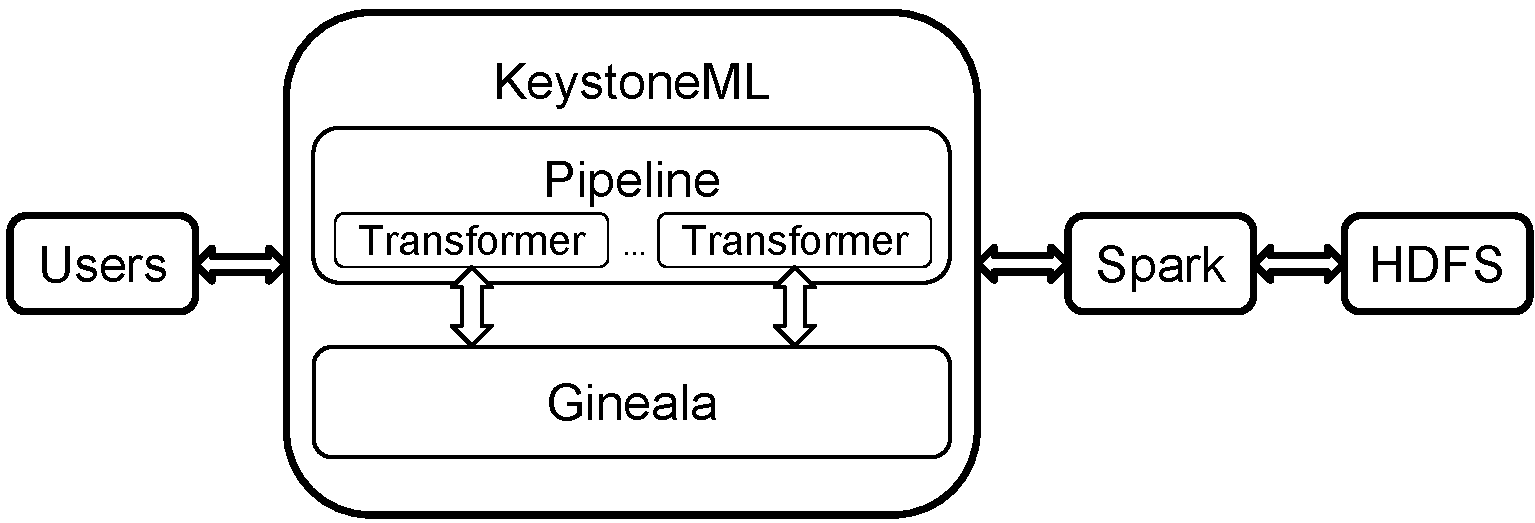
\includegraphics[width=85mm]{pictures/architecture}
\caption {Gineala's interaction with other components.
    \label{fig:architecture}
}
\end{center}
\end{figure}

\section{Implementations}
\label{sec:Impl}

\subsection{Metadata}

\subsection{Index}

\subsection{Replay}

\section{Performance Measurements}
\label{sec:Perf}
Measurements

\subsection{Overhead}
Overhead

\subsection{Query}
Query

\subsection{Replay}
Replay

\subsection{Use Case}
Query

\section{Related Work}
\label{sec:Related}
Related work

\section{Conclusion and Future Work}
\label{sec:Conclusion}
Conclusion

%ACKNOWLEDGMENTS are optional
\section{Acknowledgments}
This research is supported in part by NSF CISE Expeditions Award CCF-1139158, LBNL Award 7076018, and DARPA XData Award FA8750-12-2-0331, and gifts from Amazon Web Services, Google, SAP,  The Thomas and Stacey Siebel Foundation, Adatao, Adobe, Apple, Inc., Blue Goji, Bosch, C3Energy, Cisco, Cray, Cloudera, EMC, Ericsson, Facebook, Guavus, Huawei, Intel, Microsoft, NetApp, Pivotal, Samsung, Splunk, Virdata, VMware, and Yahoo!. Author FAN is supported by a National Science Foundation Graduate Research Fellowship.

%
% The following two commands are all you need in the
% initial runs of your .tex file to
% produce the bibliography for the citations in your paper.
\bibliographystyle{abbrv}
\bibliography{Lineage} % sigproc.bib is the name of the Bibliography in this case
% You must have a proper ".bib" file
%  and remember to run:
% latex bibtex latex latex
% to resolve all references
%
% ACM needs 'a single self-contained file'!
%
%APPENDICES are optional
%\balancecolumns



\balancecolumns

% That's all folks!
\end{document}
